% !TEX root = mainthesis.tex
%Chapter 8

\renewcommand{\thechapter}{8}

\chapter{Unconventional topology with a Rashba SOC quantum gas}
\label{ch:Rashba}

Engineering non-abelian gauge fields 
talk a bit about the background. Why rashba is interesting and why did we choose to to this with Rashba. 
This work started as Rashba but our attention was quickly shifted towards topology. We did this because we wanted to something that 

The topology of Bloch bands defines integers that serve to both classify crystalline materials and precisely specify properties, such as conductivity, that are independent of small changes to lattice parameters\cite{hasan_colloquium:_2010}. Topologically non-trivial materials first found application in metrology with the definition of the von Klitzing constant as a standard of resistance, which is now applied in the realization of the kilogram\cite{newell_codata_2018}. Today, topological systems have found applications in the engineering of low loss optical waveguides\cite{ozawa_topological_2019} and present a promising path to quantum computation\cite{nayak_non-abelian_2008}. Ultracold atomic systems are an emerging platform for engineering topological lattices, from the Harper-Hofsdater model\cite{miyake_realizing_2013,aidelsburger_realization_2013}, the Haldane model\cite{jotzu_experimental_2014}, to the Rice-Mele model\cite{lu_geometrical_2016,lohse_thouless_2016} as well as assembling spin-orbit coupled lattices without analogues in existing materials\cite{wu_realization_2016,sun_highly_2018}.

A central tenet in topological matter is the existence of integer valued `invariants' that are independent of small changes to parameters. For an arbitrary closed 2-manifold $\mathcal{M}$ and a suitable choice of vector field (i.e., a two-form) $\mathbf{\Omega}$ the surface integral
%
\begin{equation}
	\frac{1}{2\pi}\int_{\mathcal{M}}\mathbf \Omega\cdot d\mathbf S
	\label{Eq:topology}
\end{equation}
%
serves to define both the Euler characteristic and the Chern number \cite{ozawa_topological_2019,cooper_topological_2019}. When $\mathbf{\Omega}$ is equal to the local Gaussian curvature of $\mathcal{M}$, Equation~\ref{Eq:topology} yields the Euler characteristic, an invariant related to the number of handles, or genus, of $\mathcal{M}$. In contrast, when $\mathcal{M}$ is a torus describing a two-dimensional Brillouin zone (BZ) and $\mathbf{\Omega}$ is the Berry curvature that characterizes the underlying quantum states, Equation~\ref{Eq:topology} instead gives the Chern number. Both the Euler characteristic and the Chern number are integer valued, but the Euler characteristic depends only on the manifold $\mathcal{M}$ and its intrinsic curvature, whilst the Chern number depends both on a manifold (the BZ) and an additional vector field defined on $\mathcal{M}$ (the Berry curvature). 



Ultracold atomic systems are an emerging platform for engineering topological lattices, from the Harper-Hofsdater model\cite{miyake_realizing_2013,aidelsburger_realization_2013}, the Haldane model\cite{jotzu_experimental_2014}, to the Rice-Mele model\cite{lu_geometrical_2016,lohse_thouless_2016} as well as assembling spin-orbit coupled lattices without analogues in existing materials\cite{wu_realization_2016,sun_highly_2018}. 


Experimental realizations of topological materials have focused on engineering different Berry curvatures in lattice systems, where $\mathcal{M}$ is always a torus. Here we show that by eliminating the lattice potential and thereby changing  $\mathcal{M}$ from ${\mathbb T}^2$ to ${\mathbb R}^2$, i.e. from a torus to a Cartesian plane, it is possible to create topological branches of the dispersion relation with half-integer Chern number. In our experiments we created both topological and non-topological dispersion branches by introducing Rashba-like spin-orbit coupling (SOC)\cite{campbell_realistic_2011, huang_experimental_2016, meng_experimental_2016} to a cold quantum gas. 


To avoid confusion, in this Chapter I will use the numbers $1,2,3$ to label the cartesian coordinates $\ex, \ey, \ez$ and the letters $x,y,z$ to label dressed state parameters. 

 In the second section I will describe a series of experiments that we performed to engineer and characterize the topology of a Rashba spin-orbit coupled quantum gas. First I describe the engineering of the Rashba Hamiltonian using a trio of Raman coupled CDD states (Chapter~\ref{ch:clock_states}) and validate our engineering using Fourier transform spectroscopy (Chapter~\ref{ch:Fourier_spectroscopy}). Finally I describe a quantum state tomography procedure to measure the quantum states of our system, and directly obtain the Chern number for both a topologically trivial, where it is zero, and non-trivial configurations, where it takes half integer values. 





\section{Experimental implementation of Rashba SOC}

 We implemented the ring-coupling scheme and thereby engineered Rashba SOC by resonantly coupling three internal atomic states using two-photon Raman transitions\cite{campbell_rashba_2016} as depicted in Figure~\ref{fig:Schematic}. As shown in Figure~\ref{fig:Schematic}a, the engineered system consisted of an effective spin-1/2 Rashba subspace, along with a topologically trivial high-energy branch. Our engineered Rashba system had a single Dirac cone near $\q=0$, where the two lower dispersion branches become degenerate and the Berry curvature becomes singular. Each of these branches extend to infinite momentum, making the supporting manifold a plane rather than a torus. We characterized this system using both spectroscopy and quantum state tomography. This allowed us to measure the dispersion branches and directly observe the single Dirac point linking the lowest two branches as well as to reconstruct the Berry connection to derive the associated Chern numbers. \note{TODO:maybe the stuff of plane and torus doesn't go here}


%%%%%%%%%%%%%%%%%%%%%%%%%%%%%%%%%%%%%%%%%%%%%%%%%%%%%%%%%%%%%%%%%%
%
% Brief descrpiption of Rashba SOC: theory and implementation
%
%%%%%%%%%%%%%%%%%%%%%%%%%%%%%%%%%%%%%%%%%%%%%%%%%%%%%%%%%%%%%%%%%%

\begin{figure*}[htb]
\begin{center}
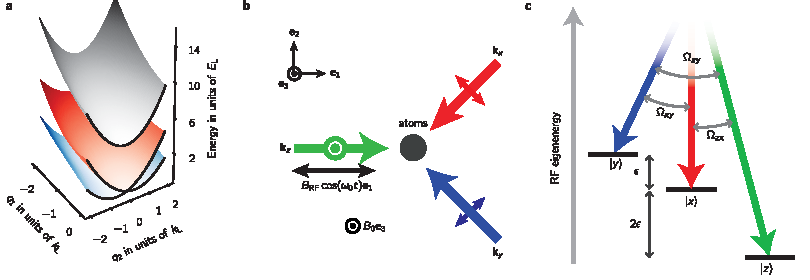
\includegraphics[width=\textwidth]{Figures/Chapter8/fig1.pdf}
\caption{{\bfseries a} Our engineered dispersion consisted of a two-level Rashba subspace (red and blue) with a single Dirac point linking the lowest two branches and a topologically trivial higher branch (gray). {\bfseries b} We generated $\xyz$ states by combining a bias magnetic field along $\mathbf{e}_3$ with an RF magnetic field oscillating along $\mathbf{e}_1$. These states were coupled by three cross-polarized Raman laser beams propagating along $\mathbf{e}_1$, $\mathbf{e}_2-\mathbf{e}_1$ and $-\mathbf{e}_1-\mathbf{e}_2$. {\bfseries c} Each pair of Raman lasers was in two-photon resonance with a single transition between the $\xyz$ states which we coupled strengths $(\Omega_{zx}, \Omega_{xy}, \Omega_{yz})/2\pi=\unit[(12.6(5), 8.7(8), 10(1))]{kHz}$.}
\label{fig:Schematic}
\end{center}
\end{figure*}

%%%%%%%%%%%%%%%%%%%%%%%%%%%%%%%%%%%%%%%%%%%%%%%%%%%%%%%%%%%%%%%%%%
%
% Brief details on experimental implementation
%
%%%%%%%%%%%%%%%%%%%%%%%%%%%%%%%%%%%%%%%%%%%%%%%%%%%%%%%%%%%%%%%%%%

All of our experiments started with about with $N\approx 1\times 10^6$$\Rb87$ atoms in a crossed optical dipole trap\cite{lin_rapid_2009}, with frequencies $(f_1,f_2,f_3) \approx \unit[(70, 85, 254)]{Hz}$, just above the transition temperature for Bose-Einstein condensation. We initially prepared the atoms in the $\ket{F=1, m_F=-1}$ state of the $5S_{1/2}$ electronic ground state and transfered atoms to the $m_F=0$ and $m_F=+1$ states as needed using ARP. A bias field $B_0\mathbf{e}_3$ gave a $\omega_0/2\pi=\unit[23.9]{MHz}$ Larmor frequency along with a quadratic shift of $\epsilon/2\pi=\unit[83.24]{kHz}$. The experiments were performed using the $\xyz$ states described in Chapter~\ref{ch:clock_states}. We implemented CDD using an RF magnetic field oscillating at the Larmor frequency with strength $\Omega_{\rm RF}=1.41(2)\epsilon$. We adiabatically prepared the $\xyz$ states starting from the $m_F$ states following the procedure described in Chapter~\ref{sec:xyz_state_preparation}. 

\subsection{Raman coupling the $\xyz$ states}

We Raman-coupled atoms prepared in any of the $\xyz$ states using the three cross-polarized Raman laser beams shown in Figure~\ref{fig:Schematic}b, tuned to the `magic zero' wavelength $\lambda_L = \unit[790]{nm}$. We arranged the Raman lasers into the tripod configuration shown in Figure~\ref{fig:Schematic}c, bringing each pair into two-photon resonance with a single transition with strengths $(\Omega_{zx}, \Omega_{xy}, \Omega_{yz})/2\pi=\unit[(12.6(5), 8.7(8), 10(1))]{kHz}$. 

The energies of the $\xyz$ states are $\omega_x=0$ and $\omega_{z,y}=-(\epsilon\pm\sqrt{4\Omega_{\rm RF}^2+\epsilon^2})/2$. We set the frequencies of the Raman lasers to $\omega_x=\omega_L+\omega_0+\omega_{xy}$, $\omega_y=\omega_L+\omega_0$ and $\omega_z=\omega_L-\omega_{zx}$,  where $\omega_L=2\pi c/\lambda_L$ and $(\omega_{zx}, \omega_{xy}, \omega_{zy})/2\pi = \unit[(166.47, 83.24, 249.71)]{kHz}$ are the transition frequencies between pairs of dressed states and are integer multiples of $\epsilon$ for our coupling strength $\Omega = \sqrt{2}\epsilon$. 

The Raman coupled states are well described by the combined kinetic and light-matter Hamiltonian
%
\begin{equation}
	\hat H(\k) =\sum_{j\in\{xyz\}}\bigg(\frac{\hbar^2k^2}{2m}+\hbar \omega_i\bigg)\ket{j}\bra{j}+\sum_{j'\neq j}\hbar\Omega_{j,j'}e^{i(\k_{j,j'}\cdot\x-i\omega_{j,j'}t)}\ket{j}\bra{j'},
	% \label{Eq:Rashba_atoms}
\end{equation}
%
where $\k_{j,j'}$ is the recoil momentum from an $\ket{j}\rightarrow\ket{j'}$ transition and $\Omega_{ij}$ is the Raman coupling strength between a pair of RF dressed states. The Hamiltonian above only includes the matrix elements associated to resonant couplings. We then apply the unitary transformation $\hat{U}_{j,j'}=\exp(-i\k_j\cdot\x-\omega_j t)\delta_{j,j'}\ket{j}\bra{j'}$ so that the Hamiltonian takes the familiar form of the ring coupling scheme
\begin{equation}
	\hat H(\q) =\sum_{j\in\{xyz\}}\bigg(\frac{\hbar^2(\q-\k_j)^2}{2m}+\hbar\delta_j\bigg)\ket{j}\bra{j}+\sum_{j\neq j'}\hbar\Omega_{jj'}\ket{j}\bra{j'},
	\label{Eq:Rashba_atoms}
\end{equation}
%
where $\k_j$ are the Raman wave vectors and $\delta_j$ is the detuning from Raman resonance.

This coupling scheme simultaneously overcomes three limitations of earlier experiments\cite{huang_experimental_2016,meng_experimental_2016} that performed the ring coupling using a combination of states in the $F=1$ and $F=2$ hyperfine manifolds of $^40$K : (1) working in the same hyperfine manifold eliminates spin-relaxation collisions; (2) unlike $m_F$ states, the $\xyz$ states can be tripod-coupled with lasers far detuned relative to the excited state hyperfine splitting greatly reducing spontaneous emission\cite{cooper_reaching_2013}; and (3) CDD renders the $\xyz$ states nearly immune to magnetic field noise.
\note{TODO: understand what is the deal with spin-relaxation collisions}

\subsubsection{Lifetime}

The measured spontaneous emission limited lifetime of our system is $\unit[320(17)]{ms}$. However it is reduced to $\unit[40(2)]{ms}$ when the Raman couplings are resonant, which we attribute to technical noise in the relative phase between the RF dressing field and the Raman laser fields, which has caused considerable consternation in ongoing experiments. However annoying this reduced lifetime is, all the experiments reported here were short compared to the lifetime and this was not an issue. Figure~\ref{fig:raman_lifetime} shows the integrated OD from TOF images of thermal atoms where the Raman was turned on in $\unit[1]{ms}$ and held on for up to $\unit[50]{\mu s}$. 

\begin{figure*}[htb]
\begin{center}
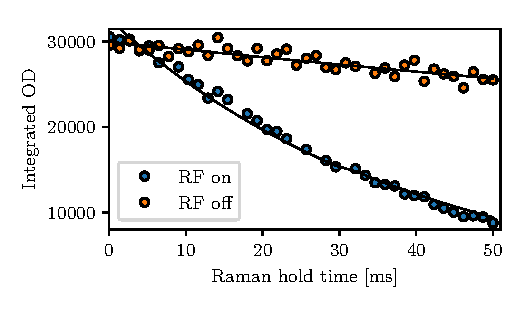
\includegraphics[]{Figures/Chapter8/raman_lifetime.pdf}
\caption[Lifetime of Raman dressed states]{Lifetime of Raman dressed states. We Raman dressed atoms in the $\ket{m_f}$ and $\xyz$ states. The orange markers correspond to atoms initially prepared in $\ket{m_f=-1}$ (no high power RF involved) and the blue markers correspond to atoms $\xyz$ (three averaged traces). The lifetime of doubly dressed states is significantly reduced as compared to the lifetime of the Raman dressed $\ket{m_f}$ states, indicating that of resonant scattering of photons is not our only loss mechanism.}
\label{fig:raman_lifetime}
\end{center}
\end{figure*}

\subsubsection{Floquet and off resonant coupling effects}

We operated in a regime where the transition energies between the $\xyz$ states were integer multiples of $\omega_{xy}$: $\omega_{zx}=2\omega_{xy}$ and $\omega_{zy}=3\omega_{xy}$, and therefore we can use Floquet theory for a complete description of our system\cite{goldman_periodically_2014}. The Hamiltonian in Equation~\ref{Eq:Rashba_atoms} is therefore an effective Hamiltonian that describes the stroboscopic dynamics of the full Floquet Hamiltonian. We observed that the effective Raman coupling strengths for the driven three level system differed from our calibrations which were performed by only driving one pair of states because of the presence of nearby quasi-energy manifolds. This effect could be mitigated for larger values of $\omega_{xy}$ as the spacing between quasi-energy manifolds is increased. Appendix~\ref{app:rashba_derivation} has a full derivation of the Raman Hamiltonian starting from the $\ket{m_F}$ basis in the lab frame including the full time dependence and off resonant terms. 

\begin{figure*}[htb]
\begin{center}
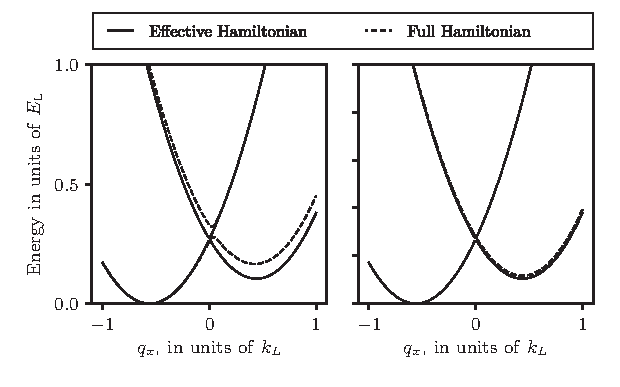
\includegraphics[]{Figures/Chapter8/floquet_effects_legend.pdf}
\caption[Effect of neighboring Floquet manifolds on Rashba dispersion]{Solid lines: Dispersion relation from the effective Floquet Hamiltonian from Equation~\ref{Eq:Rashba_atoms} as a function of $q_x$ for $\Omega_{i,j}=\unit[1.5]{\El}$ and $\delta_i=0$. Dashed lines: Dispersion relation computed for the full Floquet Hamiltonian. We considered $\omega_{zx}=2\omega_{xy}$ and $\omega_{zy}=3\omega_{xy}$ in both cases so the separation between Floquet manifolds is $\omega_{xy}$. In the left panel $\omega_{xy}=\unit[83.24]{kHz}$ as in our experiments and in the right panel $\omega_{xy}=\unit[416.2]{kHz}$. As the spacing between Floquet manifolds becomes larger, the dispersion from the effective and full Hamiltonians become closer.}
\label{fig:floquet_effects}
\end{center}
\end{figure*}

\subsection{Measuring quasimomentum distributions}
Each pair of Raman lasers coupled states $\ket{i, \k}\rightarrow \ket{j, \k+\k_{i,j}}$ where $\ket{i}$ and $\ket{j}$ denote the initial and final $\xyz$ states, $\k$ is the initial momentum and $\k_{i,j}=\k_i-\k_j$ is the two-photon Raman recoil momentum. Dressed states with quasimomentum $\q$ are comprised of three bare states $\ket{j,\k}$ with momentum $\k=\q-\k_j$. The eigenstates of our Rashba SOC Hamiltonian take the form
\begin{equation}
	\ket{\Psi_n(\q)}=\sum_{j\in xyz}\sqrt{a_{n,j}(\q)}e^{i\phi_{n,j}(\q)}\ket{j,\k=\q-\k_{j}},	
	\label{Eq:Raman_wavefunction}.
\end{equation}
where the quasimomentum $\q$ is a good quantum number and the amplitudes are parametrized by $a_{n,j}(\q)$ and $\phi_{n,j}(\q)$. We leveraged the wide momentum distribution of a non-condensed ensemble ($T\approx\unit[180]{nK}$ and $T/T_c\approx 1.1$) to sample a wide range of momentum states simultaneously. By starting separately in each of the $\xyz$ states we sampled the range of quasimomentum states shown in Figure~\ref{fig:fourier_spectroscopy}a, where the momentum distributions of an initial state $\ket{j,\k}$ is shifted from $\q=0$ by the corresponding Raman wave vector $\k_{j}$. 

Our measurement protocol consisted of abruptly removing the confining potential and the Raman lasers, initiating a $\unit[21]{ms}$ TOF. During this TOF we adiabatically transformed each of the $\xyz$ states back to a corresponding $\ket{m_F}$ state following the same procedure described in Chapter~\ref{sec:xyz_state_preparation} and spatially separated them using a Stern-Gerlach gradient. Finally we used resonant absorption imaging to measure the resulting density distributions.

The FWHM of the cloud after TOF is $\unit[700]{\mu m}$ which is much larger than the size of the in-situ cloud $\sim\unit[50]{\mu m}$ and therefore the spatial density distribution of the TOF images represents momentum distribution of the atoms.  For the $\unit[7.4]{\mu m}$ pixel size of our camera and the $3.283$ magnification of our imaging system, the momentum resolution of our images was $\unit[0.018]{\kl}$ and the momentum distributions after TOF had a FWHM of $\sim\unit[2.2]{\kl}$. 

\subsubsection{Correcting shears from gradients}

The SG field had a non-zero curvature which caused a compression (or expansion) of the $m_f=-1\ (+1)$ cloud in the direction perpendicular to the SG direction. The projections of a given momentum state $\k$ along the SG axis and perpendicular to it were transformed as $k_{\parallel}\rightarrow k_{\parallel}$ and $k_{\perp}\rightarrow (1+\alpha)k_{\perp}$, where $\alpha=0$ for $m_f=0$ and $\mathrm{sign}(\alpha)=\pm 1$ for $m_f=\pm 1$. Since all our measurements were momentum dependent we had to take special care to quantify and correct this effect on the TOF images. 

We used two different methods to quantify these shears. First we prepared thermal atoms in all three of the $m_f$ states and fit 2D Gaussians rotated by the angle of the SG displacement; $63.8$ degrees for our images. Figure~\ref{fig:sg_shear} shows the standard deviation extracted from the Gaussian fits along the axis perpendicular to the SG deviation as a function of $m_f$ state. We performed a liner fit of $\sigma$ and found that the $m_f=\pm$ states are expanded/contracted by about $\pm 6.7\%$. 

\begin{figure*}[htb]
\begin{center}
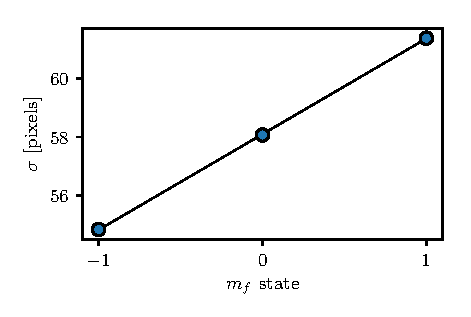
\includegraphics[]{Figures/Chapter8/sg_shear.pdf}
\caption{Averaged for 10 shots. $\alpha\approx0.067$}
\label{fig:sg_shear}
\end{center}
\end{figure*}

Alternatively we performed the Ramsey interferometer described in Section~\ref{sec:Ramsey} but coupling only 2 states, either $\ket{z}\leftrightarrow\ket{x}$ or $\ket{x}\leftrightarrow\ket{y}$ (mapped to $\ket{-1}\leftrightarrow\ket{0}$ and $\ket{0}\leftrightarrow\ket{+1}$ after TOF). We looked at the oscillation frequencies on each pixel and fit them to Equation~\ref{eq:ramsey_freq} for fixed value of the recoil momentum $\k_{i,j}$ and with a free shear parameter that modifies $\q$. Using this method we extracted a shearing of the order of $7\%$, in good agreement with the Gaussian fitting method.

The transformed momentum coordinates were described by a function $g(\k)=\k^{\mathrm{(shear)}}$ and our observed data $(y_i^{(\mathrm{shear})},\k^{(\mathrm{shear})})$ was the OD in the sheared coordinate system at the $i$th pixel of the CCD sensor. The OD in the unsheared coordinate system can be estimated by
%
\begin{equation}
	y_j = \frac{\sum_i\exp[-(g(\k_j)-\k_i^{\mathrm{(shear)}})^2/2\sigma^2]y_i^{\mathrm{(shear)}}}{\sum_i\exp[-(g(\k_j)-\k_i^{\mathrm{(shear)}})^2/2\sigma^2]},
\end{equation}
%
where we used $\sigma$ as the spacing between points in the unsheared coordinate sytem. Prior to any data analysis we applied this transformation to all of our images, where we used different values of $\alpha$ that define $g(\k)$ for each of the $m_f$ states.

\note{TODO: Need to understand origin of this...}
%%%%%%%%%%%%%%%%%%%%%%%%%%%%%%%%%%%%%%%%%%%%%%%%%%%%%%%%%%%%%%%%%%
%
% Results I: Fourier spectroscopy
%
%%%%%%%%%%%%%%%%%%%%%%%%%%%%%%%%%%%%%%%%%%%%%%%%%%%%%%%%%%%%%%%%%

\section{Fourier spectroscopy of the Rashba dispersion}
\begin{figure*}[htb]
\begin{center}
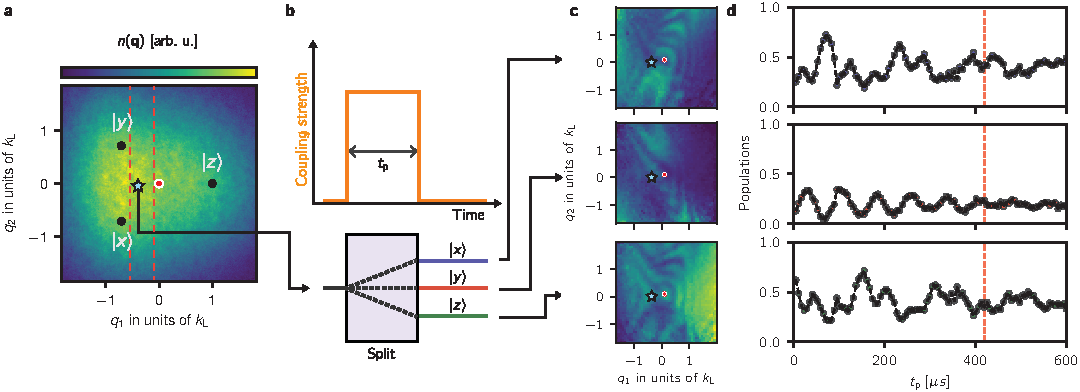
\includegraphics[width=\textwidth]{Figures/Chapter8/fig2.pdf}
\caption{{\bfseries a} The initial thermally occupied $\xyz$ states $\ket{j,\k}$ lead to the displayed quasimomentum distribution. The black dots represent $\k=0$ for each of the $\xyz$ states which is mapped to non-zero $\q$, the red dot represents $\q=0$ and the blue star indicates the quasimomentum $(q_1, q_2)=\unit[(-0.55,-0.18)]{k_{\rm L}}$. We used non-condensed atoms with a broad momentum distribution ($T\approx\unit[180]{nK}$ and $T/T_c\approx 1.1$) and performed our experiments starting separately in each of the $\xyz$ states, sampling a large range of quasimomentum states. {\bfseries b} Fourier spectroscopy protocol. We applied the Raman lasers for a variable time $t_{\mathrm{p}}$: a Rabi-type atomic interferometer analogous to a three-port beam splitter. {\bfseries c} Probabilities as a function of quasimomentum for a fixed Raman pulse time $t_{\rm p}=\unit[420]{\mu s}$ {\bfseries d} Dynamics of the final populations of the $\xyz$ states with quasimomentum $(q_1, q_2)=\unit[(-0.55,-0.18)]{k_{\rm L}}$ (red star in panels {\bfseries a} and {\bfseries c}) after initializing the system in the $\ket{z}$ state. }
\label{fig:fourier_spectroscopy}
\end{center}
\end{figure*}

We directly measured the 2D dispersion relation using Fourier transform spectroscopy\cite{valdes-curiel_fourier_2017} (see Chapter~\ref{ch:Fourier_spectroscopy}). In this technique we considered the evolution of an initial state $\ket{i,\mathbf{k}}$ suddenly subjected to the Raman coupling lasers. This atomic Rabi-type interferometer is analogous to the three-port beam-splitter depicted in Figure~\ref{fig:fourier_spectroscopy}b. During a pulse time $t_{\mathrm{p}}$ we followed the dynamics of the populations in the $\xyz$ states which evolved with oscillatory components proportional to $\sum_{j\neq n} a_{n,j}(\q)\cos([E_n(\q)-E_{j}(\q)]t_{\mathrm{p}}\,/\hbar)$, with frequencies determined by the eigenenergy differences $E_n-E_j$. Figure~\ref{fig:fourier_spectroscopy}c shows the momentum dependent populations for a fixed pulse time $t_{\mathrm{p}}$ and Figure~\ref{fig:fourier_spectroscopy}d shows representative final populations as a function of $t_{\mathrm{p}}$ for a fixed quasimomentum state. We Fourier transformed the populations with respect to $t_p$ and for a given quasimomentum state for a total of 9 state, all of them with the same $\q$ accounting for each of the three initial $\xyz$ states that was then split into 3 states. Figure~\ref{fig:fourier_grid} shows the PSD computed for each of the 9 states for planes of constant $q_1$. The amplitude of the oscillatory components depends on the overlap integral between the initial state and the Raman dressed states as was discussed in Chapter~\ref{ch:Fourier_spectroscopy} so sampling all these states gave us access to a wider range of measurable frequencies. The spectral maps in Figure~\ref{fig:fourier_spectroscopy_bands}b were produced by averaging the PSDs from the 9 different states using $\bar{n}$, the mean population in $t_{\rm p}$, as a weight:
%
\begin{equation}
	\mathrm{PSD}^{(\rm{mean})}(\q) = \frac{\sum_{i,j}\mathrm{PSD}(\q)\bar{n}_{i,j}(\q)}{\sum_{i,j}\bar{n}_i,j(\q)},
\end{equation}
%
where the indices $i,j$ represent the different states of the grid shown in Figure~\ref{fig:fourier_grid}. The extrema in the spectral maps are the energy differences $E_n-E_j$ in the engineered dispersion (Figure~\ref{fig:fourier_spectroscopy}a). The combined maps show the presence of a single Dirac point in the Rashba subspace, evidenced by the gap closing near $\q=0$ and the photon-like lower branch. The dashed curves correspond to the energy differences computed for our system using the dispersions shown in Figure~\ref{fig:fourier_spectroscopy_bands}a, and are in clear agreement with our experiment. %This measurement directly confirms the expected set of energies, including the existence of a two-state subspace approximately described by the Rashba Hamiltonian. 
\begin{figure*}[htb]
\begin{center}
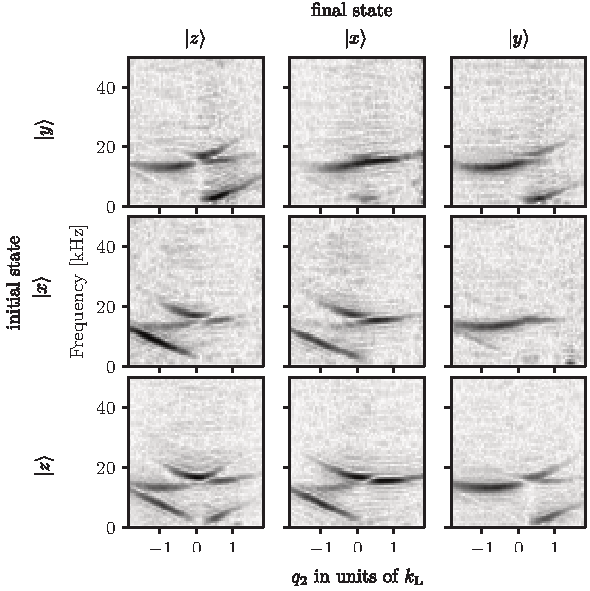
\includegraphics[]{Figures/Chapter8/fourier_grid.pdf}
\caption{Something}
\label{fig:fourier_grid}
\end{center}
\end{figure*}

\begin{figure}[htb]
\begin{center}
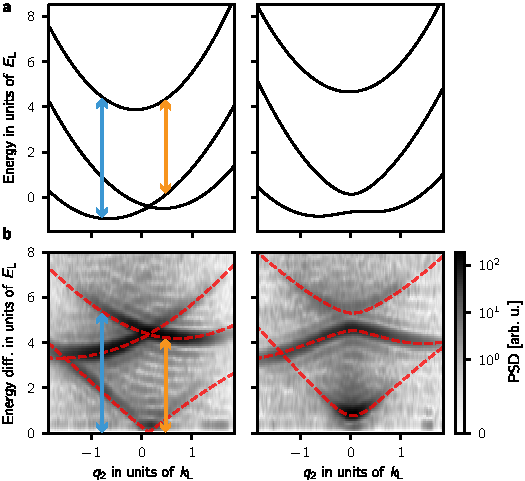
\includegraphics[]{Figures/Chapter8/fig3.pdf}
\caption{{\bfseries a} Predicted dispersion relation as a function of $q_2$ for fixed $q_1=-0.09 \,k_{\rm L}$ (left) and $0.65\,k_{\rm L}$ (right), computed for the experiment parameters. The energy differences between the branches enclosing the vertical arrows appear as peaks in the spectral maps below. {\bfseries b} Power spectral density (PSD) for the same parameters as above which we obtained by Fourier transforming the populations in the $\xyz$ states with respect to $t_{\mathrm{p}}$. The dashed lines correspond to the energy differences computed using the dispersion curves on the top panel.}
\label{fig:fourier_spectroscopy_bands}
\end{center}
\end{figure}


%%%%%%%%%%%%%%%%%%%%%%%%%%%%%%%%%%%%%%%%%%%%%%%%%%%%%%%%%%%%%%%%%%
%
% Results II: Measurement of Chern number
%
%%%%%%%%%%%%%%%%%%%%%%%%%%%%%%%%%%%%%%%%%%%%%%%%%%%%%%%%%%%%%%%%%%
%
\subsection{Quantum state tomography with Ramsey interferometer}
\label{sec:Ramsey}

The Fourier spectroscopy measurement confirmed our quantum engineering of the Rashba Hamiltonian. However, the energies shed no light on the topology of the different branches of the dispersion, which instead requires knowledge of the eigenstates. The Berry curvature present in Equation~\ref{Eq:topology} can be derived from the Berry's connection $\mathbf{A}_n(\q)=i\bra{\Psi_n(\q)}\mathbf{\nabla}_q\ket{\Psi_n(\q)}$, and using the expression for the Raman dressed eigenstates from Equation~\ref{Eq:Raman_wavefunction} we obtain

% which behaves much like a vector potential in classical electromagnetism. The Berry curvature $\mathbf{\Omega}_n(\q)=\mathbf{\nabla}_q\times\mathbf{A}(\q)$ is the associated magnetic field and the flux through any surface is the line integral of $\mathbf{A(\q)}$ along its boundary, after neglecting the contributions of Dirac strings which we will discuss later. T
%
\begin{equation}
 \mathbf A_n(\q)= -\!\!\!\!\!\!\sum_{j \in\{x, y, z\}}  a_{n,j}(\q)  \nabla_q \phi_{n,j}(\q),
\label{Eq:Berry_connection1}
\end{equation}
%
which depends on both the phase and amplitude of the wave function. We obtained $a_{n,j}(\q)$ and $\phi_{n,j}(\q)$ using a three-arm time-domain Ramsey interferometer, implementing a variant of quantum state tomography\cite{flaschner_experimental_2016,godfrin_generalized_2018}. The use of a multi-path interferometer allowed us to transduce information about phases into state populations, which we readily obtained from absorption images. 

%
\begin{figure*}[htb]
\begin{center}
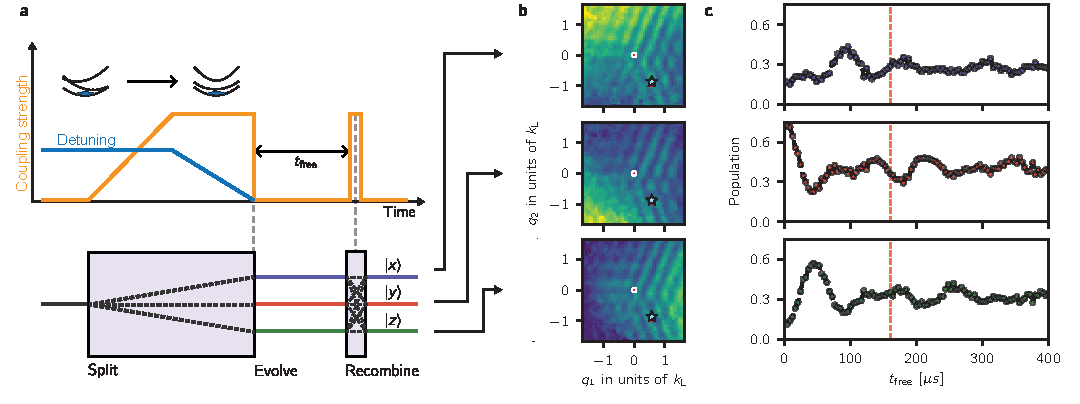
\includegraphics[]{Figures/Chapter8/fig4.pdf}
\caption{{\bfseries a} Experimental protocol for three-arm Ramsey interferometer (not to scale). (Top) We started with atoms in state $\ket{z,y,\q_i=\k+\mathbf{k}_j}$ and with detuning $\delta_y=\pm \unit[5]{E_{\rm L}}$ and $\delta_z=\pm\unit[5]{E_{\rm L}}$. We ramped the Raman lasers on in $750 \us$ and then ramped the detuning to nominally zero. We let the system evolve in the dark for times between $5 \,\us$ and $400\,\us$, followed by a $\unit[25]{us}$ Raman pulse. (Bottom) The implemented experimental protocol was equivalent to a three-arm interferometer that split an initial state into three final states with amplitudes related to the initial wave function phases. {\bfseries b} Probabilities as a function of quasimomentum for the three output ports of the interferometer at $t_{\rm free}=\unit[160]{\mu s}$ {\bfseries c} Probabilities as a function of free evolution time $t_{\mathrm{free}}$ for an input state with quasimomentum $(q_1, q_2)=(0.55,-0.92)\,k_{\rm L}$ indicated by the blue star on {\bfseries b} and in the topological ground branch ($n=1$)}
\label{fig:Ramsey_ramps}
\end{center}
\end{figure*}

Figure~\ref{fig:Ramsey_ramps}a shows our experimental protocol. We adiabatically mapped an initial $\ket{j, \k}$ state into a corresponding eigenstate $\ket{n,\q=\k+\k_j}$, either in the topologically trivial highest dispersion branch ($n=3$) or in the topological ground branch ($n=1$) by dynamically tailoring both the Raman coupling strength and detuning (see Methods). We suddenly turned off the Raman coupling, thereby allowing the three bare state components of the Rashba eigenstates to undergo free evolution for a time $t_{\mathrm{free}}$, constituting the three arms of our time-domain interferometer. Finally we applied a three-port beam splitter using a brief Raman `recombination' pulse to interfere the three arms. At the end of this procedure, the population in a final state $\ket{l, \q}$ is
\begin{equation}
P_l(\q,t)=\sum_{i\neq j} a_{n,i}a_{n,j}\cos(\omega_{i,j}(\q) t+\phi_{n,i}(\q) - \phi_{n,j}(\q)+\phi_{l,i,j}^{p}(\q)),
\label{Eq:Ramsey_evolution}
\end{equation}
which directly reads out the phase differences, independent of the output port $l$. Here $\phi_{l,i,j}^{p}(\q)$ is a smoothly varying phase imprinted by the recombination pulse and is independent of $\q$ in the limit of short, strong pulses. The angular frequencies
%
\begin{equation}
	\omega_{i,j}(\q)=\hbar \q \cdot \k_{i,j}/m + \delta_{i,j}
	\label{eq:ramsey_freq}
\end{equation}
%
result from the known free particle kinetic energy and detuning $\delta_{i,j}$ from the tripod resonance condition. Figure~\ref{fig:Ramsey_ramps}b shows the momentum-dependent populations in each output port at fixed $t_{\rm free}=\unit[160]{\mu s}$ and Figure~\ref{fig:Ramsey_ramps}c shows the populations as a function of $t_{\mathrm{free}}$ for a representative quasimomentum state $(q_1, q_2)=(0.55,-0.92)\,k_{\rm L}$. We obtained the relative phases from Equation~\ref{Eq:Ramsey_evolution} by fitting the measured populations to the sum of three cosines with the known free particle frequencies but unknown amplitudes and phases. 

Figure~\ref{fig:Ramsey_phases}a shows typical phase-maps for both the non-topological and topological branches. In the non-topological phase-maps the momentum dependence of the recombination pulse $\phi_{l,i,j}^{p}(\q)$ causes a smooth variation of the phases along the Raman recoil axes that does not affect the evaluation topological index of our system. To recover the phases $\phi_{n,j}$ of the full spinor wave function from the fits, we made the gauge choice described in the Methods.


We recovered the phases $\phi_{n,j}$ of the full spinor wave function from the relative phases obtained from the fits by choosing a particular gauge (see Methods). We then used the values of $a_{n,i}$ obtained from measuring the populations in the $\xyz$ states at $t_{\mathrm{free}}=0$ in combination with the phases of the wave function to compute the Berry connection\cite{fukui_chern_2005}. Figure~\ref{fig:Ramsey_phases}b shows the three phase differences as a function of polar angle for a loop of radius $q\approx 0.77\,k_{\rm L}$ for both the topological and non-topological branches. In addition to the smooth variations induced by the recombination which are present in both columns, the phases of the topological branch have two $\pi$ valued jumps that lead to non-zero Berry phases when the Berry connection is integrated along a closed loop in momentum space. Figure~\ref{fig:Ramsey_phases}c shows the integrated Berry phase as a function of loop radius. The largest value of $t_{\mathrm{free}}$ in the experiment limits how well we can resolve the phases of low frequencies $\omega_{ij}(\q)$ near $q=0$ as well as when two different frequencies $\omega_{ij}(\q)$ and $\omega_{i'j'}(\q)$ are close to each other, as can be seen in the high noise present in the phase-maps near $q=0$ as well as in lines where the fit frequencies become nearly degenerate. This limitation is reflected in the large variation in the Berry phase depicted in the shaded region of Figure~\ref{fig:Ramsey_phases}c near $q=0$. For loops with $q>0.4\,k_{\rm L}$ we obtain an integrated Berry phase that suggests an asymptotic Chern number of $\Phi_{\rm B}/2\pi=0.01(1)$ for the non-topological branch and $\Phi_{\rm B}/2\pi=0.5(5)$ for the topological branch. However, Berry's phase measurements including ours includes the (potential) contribution of any Dirac strings traversing the integration area. In our system, these are possible at the Dirac point $^*$, and each contributes $\pm2\pi$ to $\Phi_{\rm B}$. Even with this $2\pi$ ambiguity we are able to associated a half-integer Chern number with the topological branch, which is possible only for a topological dispersion branch in the continuum. 
\begin{figure}[htb]
\begin{center}
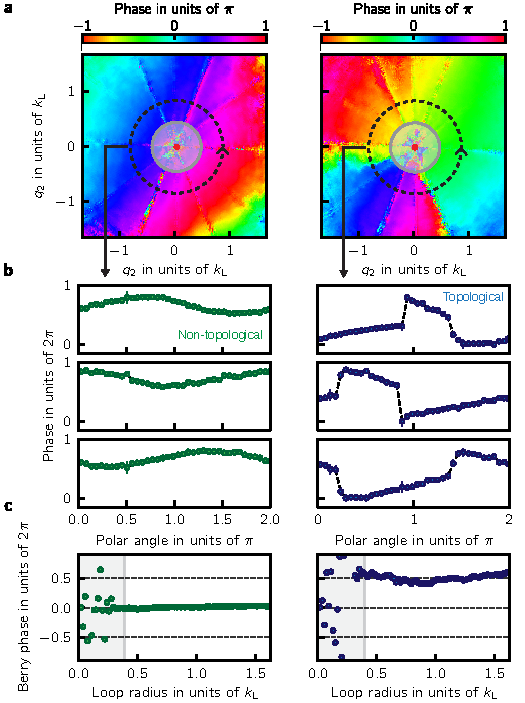
\includegraphics[]{Figures/Chapter8/fig5.pdf}
\caption{Topological invariants from quantum state tomography, for the non-topological branch ($n = 3$, left) and the topological branch ($n = 1$, right). {\bfseries a} Phase differences as a function of quasimomentum from the the $z\rightarrow x$ transition {\bfseries b} Phase differences as a function of polar angle for a loop radius $\unit[0.77]{\kl}$ from the $z\rightarrow x$ (top), $x\rightarrow y$ (middle) and $y\rightarrow z$ (bottom) transitions. The phases associated to the topological branch are characterized by two $\pi$ valued discontinuities. Each row of phases was shifted by a constant value so that the three rows of phases share the same vertical axis. All phases shown here were binned and averaged using the fit uncertainties as weights. {\bfseries c} Inferred Chern number as a function of loop radius. For loops with $q>0.4\,k_{\rm L}$ we obtained an integrated Berry phase and asymptotic Chern number of $\Phi_{\rm B}/2\pi=0.01(1)$ for the non-topological branch and $\Phi_{\rm B}/2\pi=0.5(5)$ for the topological branch.}
\label{fig:Ramsey_phases}
\end{center}
\end{figure}


In conventional lattices --- for example graphene, or the topological Haldane model --- it is well established that Dirac points each contribute a Berry's phase of $\Phi_{\rm B} /2\pi =\pm 1/2$\cite{duca_aharonov-bohm_2015}, but crystalline materials conspire for these to appear in pairs\cite{nielsen_adler-bell-jackiw_1983}, always delivering integer Chern numbers. In contrast, our continuum system contains a single Dirac point, resulting in a non-integer Chern number. This leads to intriguing questions about edge states at interfaces with non-integer Chern numbers with non-integer Chern number differences. Initial studies in the context of electromagnetic waveguides\cite{silveirinha_chern_2015 } and atmospheric waves\cite{delplace_topological_2017} have applied Chern invariants and the bulk-edge correspondence to continuous media. 

While the true Rashba Hamiltonian features a ring of degenerate eigenstates, our implementation including the quadratic and cubic Dresselhaus-like SOC lifts this macroscopic degeneracy giving three nearly degenerate minima\cite{campbell_realistic_2011}. Already these three minima could allow the study of rich ground state physics in many body systems of bosons, for example the formation of fragmented BECs\cite{stanescu_spin-orbit_2008} when the system does not condense into a single-particle state. Furthermore, the use of additional spin states or larger Raman couplings can partially restore this degeneracy allowing the possible realization of fractional Hall like states\cite{sedrakyan_statistical_2015}. 

\note{Modify words} Our present work clearly shows new non-integer values for topological invariants, but leaves open the “bulk-boundary” connection, which links quantized transport to interfaces between systems with different topological invariants.


%%%%%%%%%%%%%%%%%%%%%%%%%%%%%%%%%%%%%%%%%%%%%%%%%%%%%%%%%%%%%%%%%
%
%Methods
%
%%%%%%%%%%%%%%%%%%%%%%%%%%%%%%%%%%%%%%%%%%%%%%%%%%%%%%%%%%%%%%%%%%


%
\subsection{State preparation for Ramsey interferometer}

For the Rashba dressed states preparation we started with RF dressed states with a different coupling strength $\Omega_{\rm RF}/\pi 2\pm \unit[20]{kHz}$. This change shifted the energies of the $\ket{z}$ and $\ket{y}$ states by about $\pm \unit[18.8]{kHz}$. The change in the $\xyz$ state eigenenergies corresponded to non-zero $\delta_z$ and $\delta_y$ in Equation~\ref{Eq:Rashba_atoms}. We chose the detuning such that the initial state had a large overlap with either the $n=1$ or the $n=3$ eigenstates of Equation~\ref{Eq:Rashba_atoms}. We ramped the Raman on in $\unit[750]{\mu s}$ and then ramped $\Omega_{\rm RF}$ to its final value in $\unit[1]{ms}$, effectively ramping $\delta_z$ and $\delta_y$ close to zero. This detuning ramp had the additional effect of moving the location Dirac point through the atoms, thereby creating a trajectory where the state preparation was not adiabatic. This trajectory depended on the sign of the detuning ramp and therefore we used different initial states and detuning ramps for the ground state preparation and we excluded the Dirac point trajectories when combining the data. Near the final location of the Dirac point the state preparation can not be adiabatic regardless of the initial state or detuning used for the ground state preparation.  Finally, because of our state preparation method we could only prepare dressed states in either the $n=1$ or $n=3$ by initializing the system in the $\ket{y}$ or $\ket{z}$ states. When we prepared the system in $\ket{x}$ the final dressed state corresponded to the $n=2$ branch.


\subsection{Combining phases from different states}

The phases of the fitted populations at the output of the interferometer correspond to $\Delta\phi_{n,i,j,l}=\phi_{n,i}(\q) - \phi_{n,j}(\q)+\phi_{l,i,j}^{p}(\q)$. The last term in the expression has $\q$-independent term that depends on the final state and a $\q$-dependent term that has no dependence on the final state, i.e.,  $\phi_{l,i,j}^{p}(\q)=\phi^{p_0}_l+\phi^{p_1}_{i,j}(\q)$. When combining the phases from different initial states we removed their final state dependence by shifting $\Delta\phi_{n,i,j,l}$ by a constant number such that they maximally overlap, effectively making $\phi^{p_0}_l$ the same for all states. Finally, we averaged all the phase differences obtained from the fits, weighted by the inverse of the uncertainties obtained from the fitting procedure. For the topological branch data we excluded the regions away from $\q=0$ where the Dirac point was moved from the average. Finally we chose a gauge such that $\phi_1(\q)=0$ and used this to convert phase dif


%%%%%%%%%%%%%%%%%%%%%%%%%%%%%%%%%%%%%%%%%%%%%%%%%%%%%%%%%%%%%
%
%Graveyard
%
%%%%%%%%%%%%%%%%%%%%%%%%%%%%%%%%%%%%%%%%%%%%%%%%%%%%%%%%%%%%%
% \textit{Fiber bundles} A manifold is a topological space which looks locally like $R^n$ , but not necessarily so globally. A fibre bundle is, so to speak, a topological space which looks locally like a direct
% product of two topological spaces. 

